\documentclass[a4paper]{hitec}
\settextfraction{0.95}      % reduce left margin

\usepackage{styles/main}
\usepackage{styles/custom}
\usepackage{pdfpages}

\labtitle{Spannungs-Stabilisierung / -Quelle}

\author{Rene Hampölz, Gruppe 6}
\company{HTBLA Weiz, 5BHET}
\date{17. Oktober 2022}

% TODO: Add to Template
\newcommand{\var}[1]{\sage{norm(#1)}}

\begin{document}
\begin{sagesilent}
    load_attach_path("../helpers/")
    load("norm.sage")
    load("measures.sage")
    load("bode.sage")
\end{sagesilent}

\maketitletoc
\clearpage

\section{Einführung}

Es soll eine einfache Spannungsstabilisierung mit einer Emitterschaltung dimensioniert und aufgebaut werden.
Mit einer Simulation soll die Funktionsweise der Schaltung überprüft werden.

\begin{sagesilent}
    U_e0 = 10 
    I_a_max = 0.05
    I_Z = 0.001

    U_Z = 5.1
    U_Z_max = 5.4
    U_BE = 0.66
\end{sagesilent}

Angaben: $U_{e0} = \var{U_e0}V$, $I_{a_{max}} = \var{I_a_max}A$, $I_{Z} = \var{I_Z}A$

Datenblatt: $U_Z = \var{U_Z}V$, $U_{Z_{max}} = \var{U_Z_max}V$, $U_BE = \var{U_BE}V$

\section{Schaltung}

\begin{figure}[H]
    \centering
    \begin{circuitikz}
        \draw
        (0,0)       coordinate (in+)
        (0,-5)      coordinate (in-)
        ++(4,0)     coordinate (out-)

        (in+)           to[short,o-]                        ++(2,0) coordinate (aux1)
                        to[R=$R_1$,*-*]                     ++(0,-2) coordinate (aux2)
                        to[zD=$ZD$,i>^=$I_Z$,invert,*-*]    (aux2 |- in-)
        (aux2) ++(2,0)  node[npn]                           (T) {}
        (aux2)          to[short, i=$I_B$]                  (T.B)
        (aux1)          to[short]                           (aux1 -| T.C) -- (T.C)
        (T.E)           to[R=$R_L$,i>^=$I_a$,o-o]           (out-)
        (in-)           to[short,o-]                        (out-)

        (T.E) coordinate (out+)

        (in+)               to[open, v=$U_{e0}$]    (in-)
        ($(out+) + (1,0)$)  to[open, v^=$U_a$]      ($(out-) + (1,0)$)
        ;
    \end{circuitikz}
\end{figure}

\section{Berechnungen}

\subsection{Vorwiderstand $R_1$}

Um den von der Z-Diode benötigten Strom $I_Z$ zu liefern und um den Arbeitspunkt einzustellen, wird der Vorwiderstand $R_1$ benötigt.
Die Eingangsspannung $U_{e0}$ fällt somit an der Z-Diode sowie am Vorwiderstand $R_1$ ab:

\begin{sagesilent}
    U_R_1 = U_e0 - U_Z
\end{sagesilent}

\begin{align*}
    U_{R_1} &= U_{e0} - U_Z \\
    U_{R_1} &= \var{U_e0} - \var{U_Z} \\
    U_{R_1} &= \var{U_R_1}V
\end{align*}

Der Strom, welcher durch den Vorwiderstand $R_1$ fließt, setzt sich aus dem Strom $I_Z$ der Z-Diode und dem Basis-Strom $I_B$ des Transistors zusammen.
Der Basis-Strom $I_Z$ ist jedoch meist so klein, dass dieser vernachlässigt werden kann.

Nach dem Ohmschen Gesetz ergibt sich somit der Vorwiderstand $R_1$:

\begin{sagesilent}
    R_1 = U_R_1 / I_Z # + I_B (= <<) 
\end{sagesilent}

\begin{equation*}
    R_1 = \frac{U_{R_1}}{I_Z + I_B} \tag*{$I_B = \quad \ll$ \quad \textit{(vernachlässigbar)}} \\
\end{equation*}

\begin{align*}
    R_1 &= \frac{U_{R_1}}{I_Z} \\
    R_1 &= \frac{\var{U_R_1}}{\var{I_Z}} \\
    R_1 &= \var{R_1}\Omega
\end{align*}

\subsection{Minimaler Lastwiderstand $R_{L_{min}}$}

Die Zener-Spannung $U_Z$ \textit{(bzw. $U_{Z_{max}}$, da der minimale Lastwiderstand gesucht ist)} teilt sich in die Basis-Emitter-Spannung $U_{BE}$ des Transistors und in die Ausgangsspannung $U_a$ \textit{(bzw. $U_{a_{max}}$)} auf.
Daraus ergibt sich für die maximale Lastspannung $U_{a_{max}}$: 

\begin{sagesilent}
    U_a_max = U_Z_max - U_BE
\end{sagesilent}

\begin{align*}
    U_{a_{max}} &= U_{Z_{max}} - U_{BE} \\
    U_{a_{max}} &= \var{U_Z_max} - \var{U_BE} \\
    U_{a_{max}} &= \var{U_a_max}V
\end{align*}

Nach dem Ohmschen Gesetz ergibt sich schließlich der minimale Lastwiderstand $R_{L_{min}}$:

\begin{sagesilent}
    R_L_min = U_a_max / I_a_max
\end{sagesilent}

\begin{align*}
    R_{L_{min}} = \frac{U_{a_{max}}}{I_{a_{max}}} \\
    R_{L_{min}} = \frac{\var{U_a_max}}{\var{I_a_max}} \\
    R_{L_{min}} = \var{R_L_min}\Omega
\end{align*}

\section{Simulation}

\begin{figure}[H]
    \centering
    \includesvg[width=\textwidth]{images/01 Spannungs-Stabilisierung_Quelle.svg}
    \caption{Ausgangskennlinie \textbf{$U_a = f(R_L)$} der Simulation}
    \label{fig:simulation}
\end{figure}

Die Simulation konnte nicht mit der gleichen Z-Diode wie bei der Messung durchgeführt werden.
Daher weicht der Wertebereich in der Ausgangskennlinie der Simulation \textit{(Abb. \ref{fig:simulation})} etwas von dem der Messung \textit{(Abb. \ref{fig:measure})} ab.

\section{Auswertung}

\begin{sagesilent}
    measures = Measures(
        [
            '$R_L$ in $\Omega$',
            '$U_a$ in $V$', 
            '$I_a$ in $mA$'
        ], [
            ['100', '3.96', '38.2'],
            ['120', '3.96', '32.0'],
            ['130', '3.93', '29.5'],
            ['140', '3.94', '27.4'],
            ['150', '3.95', '25.7'],
            ['160', '3.94', '24.1'],
            ['170', '3.92', '22.6'],
            ['200', '3.91', '19.2'],
            ['250', '3.95', '15.6'],
            ['300', '3.98', '13.2'],
            ['400', '4.05', '10.0'],
            ['500', '4.10', '8.2'],
            ['600', '4.17', '6.95'],
            ['700', '4.22', '6.00'],
            ['800', '4.23', '5.30'],
            ['1000', '4.29', '4.30'],
            ['2000', '4.30', '2.16'],
    ])

    index_RL = 0
    index_Ua = 1
    index_Ia = 2
\end{sagesilent}

\subsection{Messwerte}

\begin{center}
    \renewcommand{\arraystretch}{1.2}
    \sage{measures.table}
\end{center}

\subsection{Grafische Darstellung}

\begin{sagesilent}
    f = list_plot(
        measures.plot_data(index_RL, index_Ua),
        color='purple',
        figsize=[5,2],
        axes_labels=['$R_L$ in $\Omega$', '$U_a$ in $V$'],
        axes_labels_size=1
    )

    f += line(
        measures.g1d_smooth(index_RL, index_Ua, sigma=0.75, connect=True),
        linestyle="--",
        color='blue'
    )
\end{sagesilent}

\begin{figure}[H]
    \centering
    \sageplot{f}
    \caption{Ausgangskennlinie \textbf{$U_a = f(R_L)$} mit gemessene Werte}
    \label{fig:measure}
\end{figure}

Die Schwankungen der Ausgangsspannung $U_a$ im Bereich von $100\Omega \to 200\Omega$ in der Ausgangskennlinie mit gemessenen Werte \textit{(Abb. \ref{fig:measure})} sind auf mögliche Störgrößen\textit{, wie Änderungen der Eingangsspannung oder Erwärmung der Bauteile,} zurückzuführen.

\subsection{Bemerkung}

Die Schaltung liefert ab dem ermittelten minimalen Lastwiederstand $R_{L_{min}}$ eine annähernd konstante und stabile Ausgangsspannung $U_a$ mit Abweichungen von wenigen Millivolt.
Bei größeren Lastwiederständen verhält sich die Spannung etwas stabiler.

\clearpage

\subsection{Verwendete Geräte}

\medskip

\begin{devicelist}
    \devicecat{Widerstands-Dekade}{2}{
        \device{ET-MTL1-RD23}{R_1}
        \device{ET-MTL1-RD29}{R_L}
    }
    \devicecat{Multimeter}{2}{
        \device{ET-MTL1-DM20}{I_a}
        \device{ET-MTL1-DM22}{U_a}
    }
    \devicecat{Z-Diode}{1}{
        \device{BZD23-C5V1}{}
    }
    \devicecat{Transistor}{1}{
        \device{BC550}{}
    }
\end{devicelist}

\vfill

\IncludeHistoryTimeline

\pagebreak

% \addcontentsline{toc}{section}{Datenblätter}

\invisiblesection{Datenblätter}
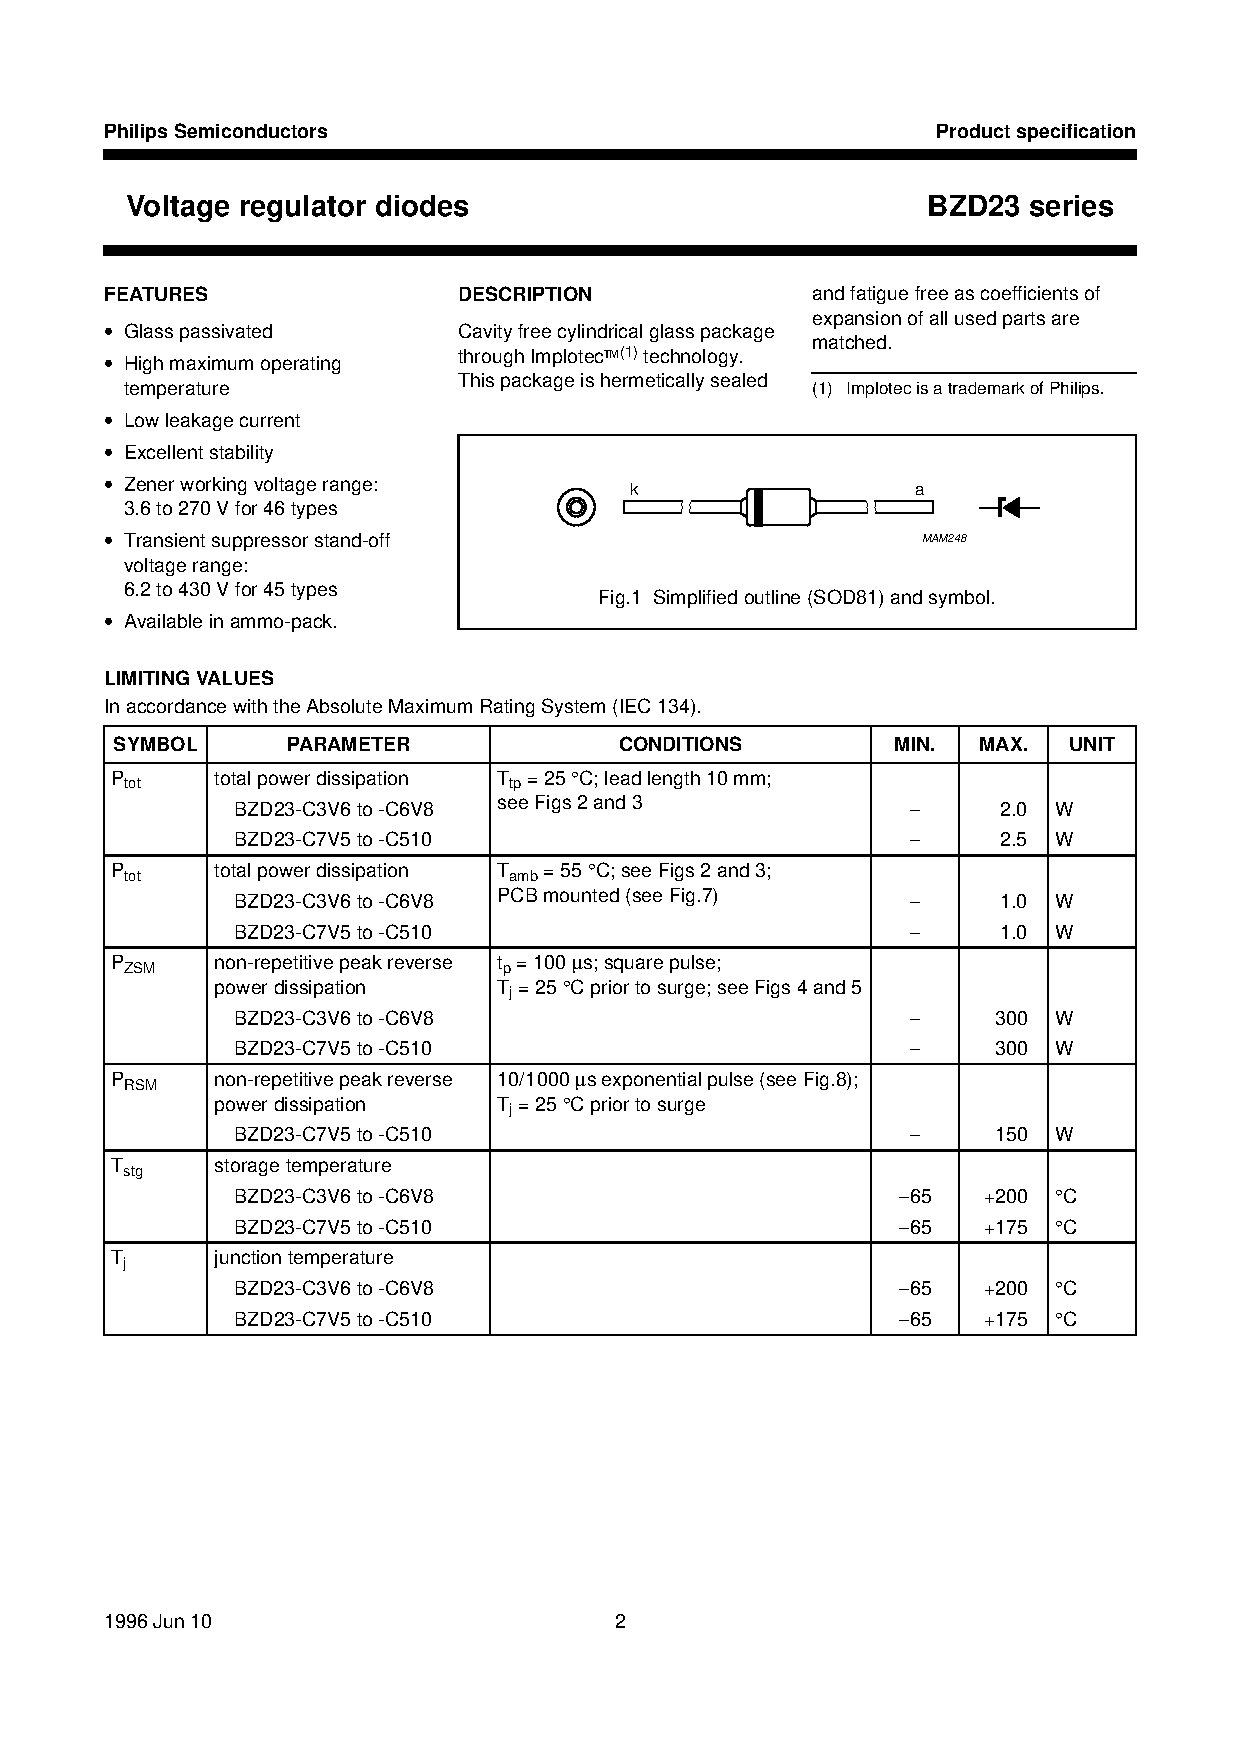
\includepdf[pages={1-}, addtotoc={1,subsection,2,BZD23-C5V1,datasheet:BZD23-C5V1}]{src/datasheets/BZD23-C5V1.pdf}
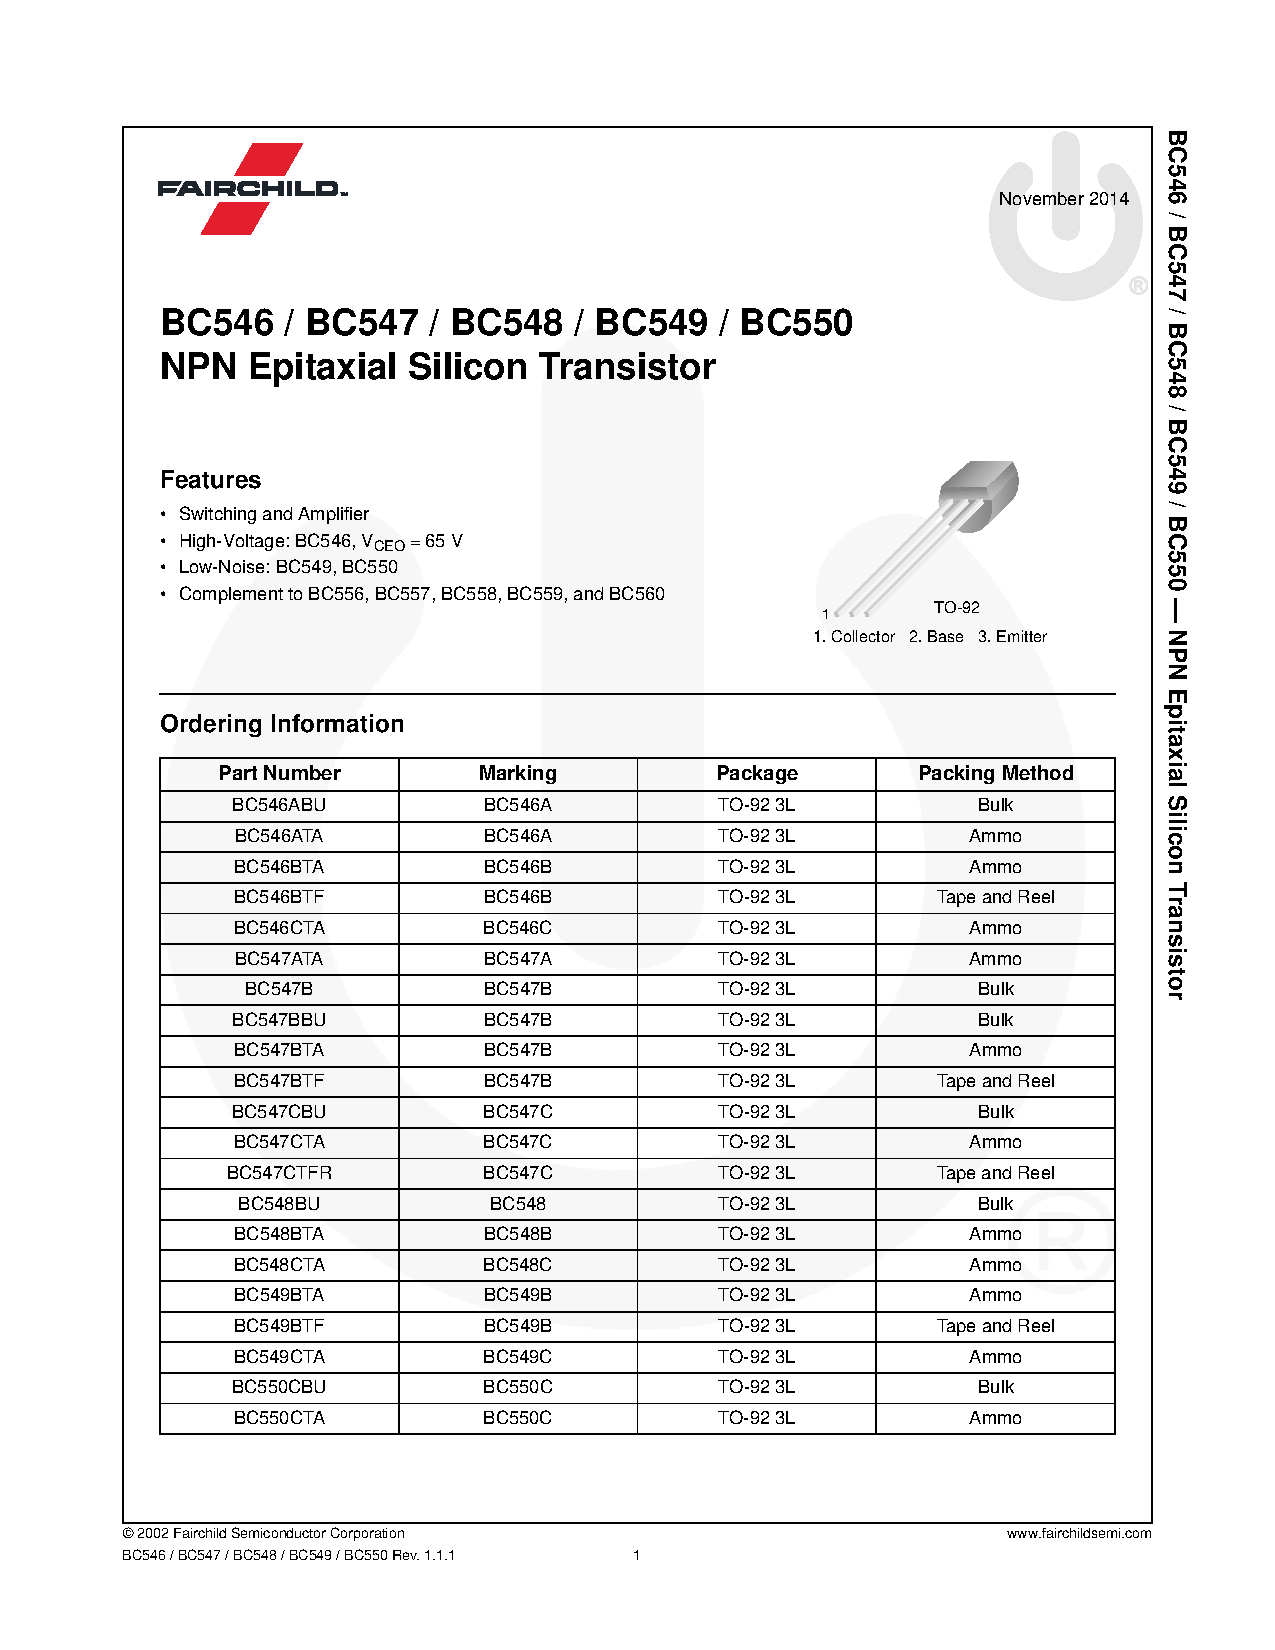
\includepdf[pages={1-}, addtotoc={1,subsection,2,BC550,datasheet:BC550}]{src/datasheets/BC550.pdf}

\end{document}